% fig_7_23.tex — 7-39: 波形曲线（某时刻一部分，标注A、B点）
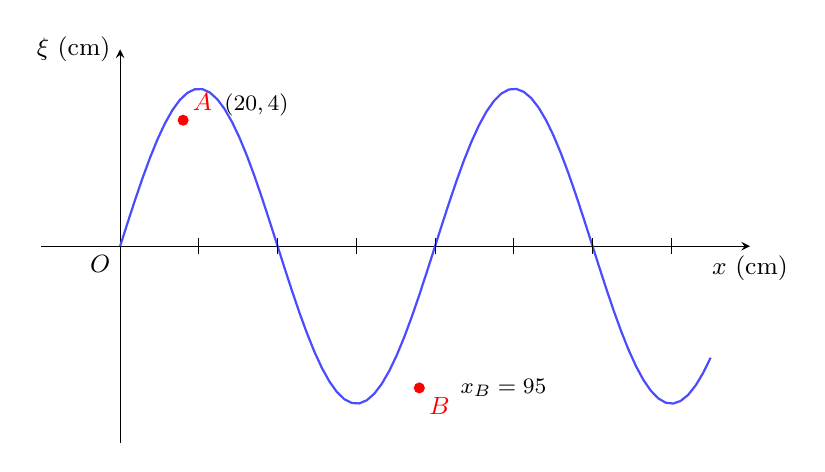
\begin{tikzpicture}[font=\small,>=stealth]
  % 坐标轴
  \draw[->] (-1,0) -- (8,0) node[below] {$x$ (cm)};
  \draw[->] (0,-2.5) -- (0,2.5) node[left] {$\xi$ (cm)};
  % 波形
  \draw[thick,blue!70] plot[domain=0:7.5,samples=80] (\x,{2*sin(deg(2*pi*\x/4))});
  % A点 (xA=20, ξA=4) → 按比例：x=20cm对应图上位置，波长100cm
  % 简化：波长λ=100cm，图上一个周期为4单位
  % A点在 x=20cm → 对应比例位置
  \fill[red] (0.8,1.6) circle (2pt) node[above right] {$A$};
  \node[font=\footnotesize,right] at (1.2,1.8) {$(20, 4)$};
  % B点 xB=95cm
  \fill[red] (3.8,-1.8) circle (2pt) node[below right] {$B$};
  \node[font=\footnotesize,right] at (4.2,-1.8) {$x_B=95$};
  % 刻度
  \foreach \x in {1,2,...,7}
    \draw (\x,0.1) -- (\x,-0.1) node[below,font=\tiny] {};
  % 原点
  \node[below left] at (0,0) {$O$};
\end{tikzpicture}
